\documentclass[11pt,a4paper]{article}
\usepackage[utf8]{inputenc}
\usepackage[T1]{fontenc}
\usepackage{lmodern}
\usepackage[margin=2.3cm]{geometry}
\usepackage{microtype}
\usepackage{xcolor}
\usepackage{booktabs}
\usepackage{tabularx}
\usepackage{enumitem}
\usepackage{listings}
\usepackage{tikz}
\usepackage{graphicx}
\usetikzlibrary{positioning,arrows.meta,fit}
\usepackage[colorlinks=true,linkcolor=blue!50!black,urlcolor=blue!50!black]{hyperref}

\definecolor{codebg}{RGB}{247,247,249}
\definecolor{todo}{RGB}{200,60,40}
\lstset{
  language=Python, basicstyle=\ttfamily\footnotesize, backgroundcolor=\color{codebg},
  keywordstyle=\color{blue!60!black}\bfseries, commentstyle=\color{green!40!black}\itshape,
  stringstyle=\color{orange!70!black}, frame=single, rulecolor=\color{black!15},
  breaklines=true, columns=fullflexible, showstringspaces=false, xleftmargin=4pt, xrightmargin=4pt
}
\newcommand{\fillin}[1]{\textcolor{todo}{\textbf{[#1]}}}
\setlist{itemsep=2pt,topsep=4pt}
%% ================== A REMPLIR / TO FILL IN ==================
\newcommand{\studentA}{\fillin{Student 1 -- matricule}}
\newcommand{\studentB}{\fillin{Student 2 -- matricule}}
\newcommand{\studentC}{\fillin{Student 3 -- matricule}}
\newcommand{\githuburl}{\fillin{GitHub URL of the repository}}
\newcommand{\nbpdfs}{\fillin{N}}
\newcommand{\llmmodel}{\fillin{llama3.2}}
\newcommand{\machine}{\fillin{Windows laptop, WSL2 Ubuntu, CPU}}
\newcommand{\sqliteoutput}{\fillin{paste output}}
\newcommand{\observations}{\fillin{Average time per paper: ... s. Number of LLM answers that needed the retry: ...}}
%% Screenshots: upload these files next to report.tex (exact names):
%%   shot1_airflow_graph.png  shot2_llm_log.png  shot3_html.png  shot4_discord.png
\newcommand{\shot}[3]{\IfFileExists{#1}{\includegraphics[width=#2\linewidth]{#1}}{\fbox{\parbox{#2\linewidth}{\centering\vspace{1.1cm}\fillin{#3}\vspace{1.1cm}}}}}
%% ===========================================================


\title{\textbf{INFO-H420 -- Assignment 3}\\[2pt]\large Workflows with Airflow: a local research-paper library pipeline}
\author{\studentA \quad \studentB \quad \studentC\\[2pt]
\small Université libre de Bruxelles}
\date{November 2026}

\begin{document}
\maketitle

\noindent\textbf{Code repository:} \githuburl\\
The repository contains the DAG, a helper module, a \texttt{README.md} with run instructions,
\texttt{requirements.txt} and \texttt{.env.example}.

\section{Goal and approach}
We built a small local pipeline that turns research PDFs into a searchable study library.
PDFs are dropped into a Google Drive-synced \texttt{papers/} folder; a scheduled Apache Airflow DAG
detects new files, converts them to Markdown, asks a \emph{locally served} LLM for structured metadata,
stores it in SQLite, regenerates a static HTML page and posts a Discord notification.

Two design decisions guided the implementation:
\begin{itemize}
  \item \textbf{Thin DAG, testable logic.} All processing code lives in \texttt{dags/library\_utils.py}
        (plain Python functions). The DAG file \texttt{dags/paper\_pipeline.py} only declares tasks
        and dependencies. The same functions can be run without Airflow (\texttt{scripts/run\_once.py}),
        which made debugging easy.
  \item \textbf{One task instance per paper.} We use Airflow \emph{dynamic task mapping}
        (\texttt{.expand()}), so each new PDF becomes an independent task instance that can be
        retried, inspected and logged separately in the UI; one faulty PDF does not block the others.
\end{itemize}
From a process-redesign perspective (Lecture~4), the pipeline applies the \emph{automation} heuristic
(H9) to a manual knowledge-work process (read, summarise, tag, file, announce), and the BPR principle
\emph{capture information once and at the source}: metadata is extracted once from the PDF itself and
stored in a single data store from which the web page and the notification are derived.

\section{Architecture}
\begin{center}
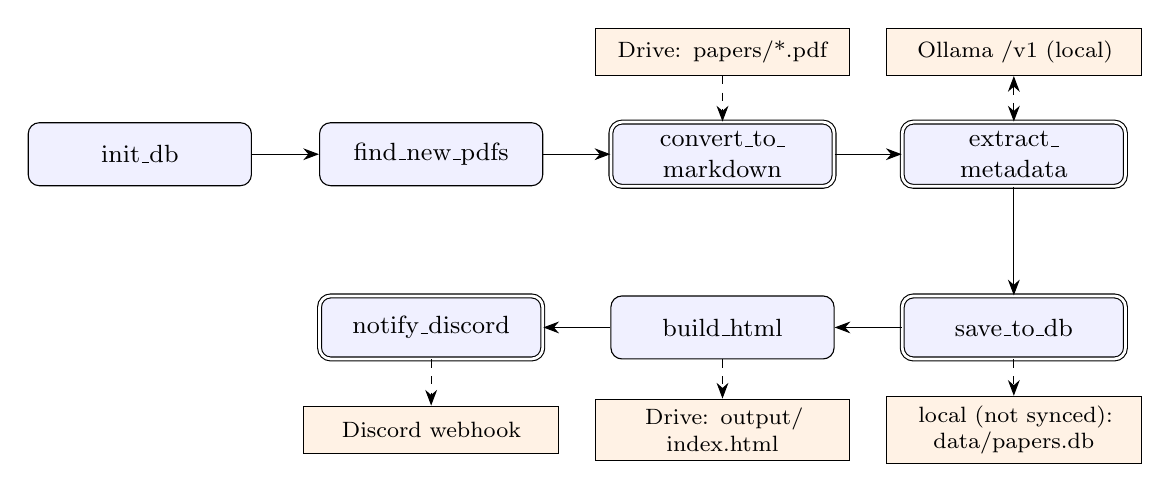
\begin{tikzpicture}[every node/.style={font=\small},
  box/.style={draw, rounded corners, fill=blue!6, minimum height=8mm, text width=26mm, align=center},
  mapped/.style={box, double, double distance=1pt},
  data/.style={draw, fill=orange!10, minimum height=6mm, text width=30mm, align=center, font=\footnotesize},
  >={Stealth[length=2mm]}]
  \node[box]    (init) at (0,0)     {init\_db};
  \node[box]    (find) at (3.7,0)   {find\_new\_pdfs};
  \node[mapped] (conv) at (7.4,0)   {convert\_to\_\\markdown};
  \node[mapped] (llm)  at (11.1,0)   {extract\_\\metadata};
  \node[mapped] (save) at (11.1,-2.2){save\_to\_db};
  \node[box]    (html) at (7.4,-2.2){build\_html};
  \node[mapped] (disc) at (3.7,-2.2){notify\_discord};
  \draw[->] (init) -- (find); \draw[->] (find) -- (conv); \draw[->] (conv) -- (llm);
  \draw[->] (llm) -- (save); \draw[->] (save) -- (html); \draw[->] (html) -- (disc);
  \node[data] (pdf) at (7.4,1.3)  {Drive: papers/*.pdf};
  \node[data] (oll) at (11.1,1.3)  {Ollama /v1 (local)};
  \node[data] (db)  at (11.1,-3.5) {local (not synced):\\data/papers.db};
  \node[data] (out) at (7.4,-3.5) {Drive: output/\\index.html};
  \node[data] (dw)  at (3.7,-3.5) {Discord webhook};
  \draw[dashed,->] (pdf) -- (conv); \draw[dashed,<->] (oll) -- (llm); \draw[dashed,->] (save) -- (db);
  \draw[dashed,->] (html) -- (out); \draw[dashed,->] (disc) -- (dw);
\end{tikzpicture}\\[2pt]
\footnotesize Double-bordered tasks are \emph{mapped}: one task instance per new PDF. Dashed arrows: external resources.
\end{center}

\noindent\textbf{Folder layout.} PDFs and \texttt{output/index.html} live in
\texttt{Google Drive/ResearchLibrary/}; the database and intermediate Markdown files stay in the local
project folder \texttt{data/}, outside the synced folder (SQLite files can be corrupted by
file-sync tools). All paths, the LLM endpoint/model and the webhook URL are configured with environment variables.

\section{Airflow DAG and task dependencies}
The DAG is written with the TaskFlow API (\texttt{@dag}/\texttt{@task}) and runs with
\texttt{airflow standalone}.
\begin{lstlisting}
@dag(dag_id="paper_pipeline", schedule=timedelta(minutes=10),
     start_date=pendulum.datetime(2026, 11, 1, tz="Europe/Brussels"),
     catchup=False, max_active_runs=1,
     default_args={"retries": 1, "retry_delay": timedelta(minutes=1)})
def paper_pipeline():
    ...
    new_files = find_new_pdfs()
    init_db() >> new_files
    docs     = convert_to_markdown.expand(filename=new_files)
    metadata = extract_metadata.expand(doc=docs)
    saved    = save_to_db.expand(metadata=metadata)
    html_page = build_html()            # trigger_rule="none_failed"
    saved >> html_page
    notifications = notify_discord.expand(metadata=saved)
    html_page >> notifications
\end{lstlisting}
\begin{itemize}
  \item \textbf{Scheduling.} Every 10 minutes; \texttt{catchup=False} avoids replaying past intervals,
        \texttt{max\_active\_runs=1} prevents two overlapping runs from processing the same PDF.
  \item \textbf{Detecting new PDFs.} \texttt{find\_new\_pdfs} compares \texttt{papers/*.pdf} with the
        filenames already stored in the database (filenames are assumed unique). The database is thus
        the single source of truth about what has been processed; no extra state file is needed.
  \item \textbf{Data passing.} Tasks exchange small values through XCom (filenames, the path of the
        Markdown file, the metadata dictionary). The Markdown text itself is written to disk, not pushed to XCom.
  \item \textbf{Empty runs.} When there is no new PDF, the mapped tasks are \emph{skipped}.
        \texttt{build\_html} uses \texttt{trigger\_rule="none\_failed"}, so it still runs and the page
        always exists; \texttt{notify\_discord} is mapped over an empty list and sends nothing.
  \item \textbf{Ordering of side effects.} Discord is notified only after the HTML page has been updated,
        so the announced paper is already visible in the library.
\end{itemize}

\section{PDF conversion and local LLM integration}
\textbf{Conversion.} \texttt{pymupdf4llm.to\_markdown()} converts each PDF; headings, lists and tables
are preserved as Markdown, which gives the LLM a clean, structured input.

\textbf{LLM call.} The model is served locally by Ollama, which exposes an OpenAI-compatible API at
\texttt{http://localhost:11434/v1} (LM Studio works by changing \texttt{LLM\_BASE\_URL}). We use the
\texttt{openai} Python package with JSON mode and a system prompt that lists the four keys and the allowed categories.
Only the first \texttt{LLM\_MAX\_CHARS} characters (default 8000: title, abstract, introduction) are sent,
to stay within the context window of small local models.
\begin{lstlisting}
client = OpenAI(base_url=LLM_BASE_URL, api_key="ollama")
response = client.chat.completions.create(model=LLM_MODEL, temperature=0.2,
    messages=[{"role": "system", "content": SYSTEM_PROMPT},
              {"role": "user", "content": "Paper (Markdown):\n\n" + text[:MAX_CHARS]}],
    response_format={"type": "json_object"})
\end{lstlisting}
\textbf{Parsing and validation.} The answer is parsed with \texttt{json.loads()}. A small validator checks
that \texttt{title}, \texttt{summary}, \texttt{category} are strings and \texttt{keywords} is a list of strings.
If parsing or validation fails, the call is \textbf{retried once}; after a second failure the task fails
with an explicit error (and Airflow's task-level retry can try again later).

\section{SQLite storage, static HTML and Discord}
\begin{itemize}
  \item \textbf{SQLite} (\texttt{sqlite3}): table \texttt{papers(filename PRIMARY KEY, title, summary,
        keywords, category, processed\_at)}; \texttt{keywords} is stored as a JSON string
        (\texttt{json.dumps}). Queries are parameterised (\texttt{?}) and \texttt{INSERT OR REPLACE} makes
        re-processing idempotent.
  \item \textbf{HTML}: \texttt{build\_html} reads all rows and rewrites \texttt{output/index.html}: one card per
        paper (title linked to \texttt{../papers/<file>.pdf}, category, summary, keywords), a search box and a
        category drop-down implemented in a few lines of plain JavaScript. All text from the LLM is
        HTML-escaped. The page is a single self-contained file, synced by Google Drive.
  \item \textbf{Discord}: \texttt{notify\_discord} sends \texttt{POST \{"content": ...\}} to the webhook
        (Discord answers \texttt{204}); it is skipped with a warning when no webhook is configured.
\end{itemize}

\section{Execution and results}
\textbf{Test set.} \nbpdfs{} PDFs placed in \texttt{ResearchLibrary/papers/}; model \llmmodel{} served by Ollama on \machine.

\begin{center}
\shot{shot1_airflow_graph.png}{0.95}{Screenshot 1: Airflow UI -- graph view of a successful run}\\[2pt]
{\footnotesize Figure 1: successful run of \texttt{paper\_pipeline} in the Airflow UI.}\\[8pt]
\shot{shot2_llm_log.png}{0.95}{Screenshot 2: log of extract\_metadata with the JSON returned by the LLM}\\[2pt]
{\footnotesize Figure 2: log of \texttt{extract\_metadata} showing the JSON returned by the local LLM.}\\[8pt]
\shot{shot3_html.png}{0.47}{Screenshot 3: index.html}\hfill
\shot{shot4_discord.png}{0.47}{Screenshot 4: Discord notification}\\[2pt]
{\footnotesize Figure 3: generated library page (left) and Discord notification (right).}
\end{center}

\noindent Output of \texttt{sqlite3 data/papers.db "SELECT filename, category FROM papers;"}:
\begin{quote}\small\ttfamily \sqliteoutput\end{quote}

\medskip\noindent\textbf{Observations.} A second run without new PDFs processes nothing and only rewrites the page
(mapped tasks skipped). \observations

\section{Limitations and possible improvements}
\begin{itemize}
  \item A file still being uploaded by Drive could be picked up half-written; a check on file age/size stability would avoid it.
  \item Only the beginning of each paper is sent to the LLM; long-document summarisation (chunking) would improve summaries.
  \item A modified PDF with the same filename is not re-processed (filenames are assumed unique, as stated in the assignment).
  \item Responsible-AI note: LLM summaries can be inaccurate; the page links to the original PDF so readers can verify.
\end{itemize}

\end{document}
